% The story of the no-op experiments, told through the figures they produced.
% Companion to noop_onepager.pdf. Every number comes from the saved runs (see ../exp2/LOOP_LOG.md).
% Build (from this folder): pdflatex noop_figure_story.tex   (twice, for the contents page)
\documentclass[10pt]{article}
\usepackage[letterpaper,margin=0.6in]{geometry}
\usepackage[T1]{fontenc}
\usepackage[scaled=0.92]{helvet}
\renewcommand{\familydefault}{\sfdefault}
\usepackage{microtype}
\usepackage{xcolor}
\usepackage{graphicx}
\usepackage{caption}
\usepackage{booktabs}
\usepackage{enumitem}
\usepackage{tikz}
\usetikzlibrary{arrows.meta,shapes.geometric}
\usepackage[hidelinks]{hyperref}
\captionsetup{font=small,labelfont=bf,justification=raggedright,singlelinecheck=false,skip=3pt}
\setlength{\parindent}{0pt}
\setlength{\parskip}{4pt}
\setlist{nosep,leftmargin=1.2em,itemsep=1pt}
\definecolor{cblue}{HTML}{2A78D6}
\definecolor{corange}{HTML}{EB6834}
\definecolor{ink2}{HTML}{52514E}
\definecolor{muted}{HTML}{898781}
\definecolor{axis}{HTML}{C3C2B7}
\definecolor{plane}{HTML}{F4F3EF}
\graphicspath{{../results/}{../../experiment_1/results/}}

% A figure in reading order (never floats away from its text): \fig{width}{path}{caption}
\newcommand{\fig}[3]{\par\begin{center}\includegraphics[width=#1\linewidth]{#2}\captionof{figure}{#3}\end{center}\par}
\newcommand{\takeaway}[1]{\par\vspace{2pt}\fcolorbox{axis}{plane}{\parbox{\dimexpr\linewidth-2\fboxsep-2\fboxrule}{\small\textbf{Takeaway.} #1}}\par\vspace{4pt}}
\newcommand{\run}[1]{{\color{muted}\scriptsize\texttt{results/#1}}}

\begin{document}

%=========================== TITLE + MAP ===========================
{\LARGE\bfseries When do GPT-2's attention heads go idle?}\\[2pt]
{\large\color{ink2} The no-op experiments, told through their figures}\\[2pt]
{\small\color{muted} Pablo Leyva \,·\, GPT-2 small \,·\, TransformerLens and Hugging Face on identical token ids \,·\, October 2026 \,·\, companion to \texttt{noop\_onepager.pdf}}

\vspace{6pt}
\textbf{The question.} At the final token of a sequence, some attention heads do work and others park their attention on the first token (BOS, the ``sink''), which acts as a \emph{no-op}. What switches a head into the no-op state? Every experiment feeds GPT-2 small a BOS token plus 32 random tokens, measures each head's attention from the final token to BOS (\emph{sink mass}), and changes the input in a controlled way.

\textbf{The story in one line per step.}
\begin{enumerate}[leftmargin=1.6em]
  \item \textbf{Experiment 1:} on random tokens, about three quarters of heads park on BOS, more so in later layers. Rare vs common tokens leave the share unchanged, but individual heads move in opposite directions.
  \item \textbf{Single-token follow-up (exp1ext):} the late-head shift comes from the whole context, and one token matters only if it sits right before the final token.
  \item \textbf{Experiment 2:} a short phrase right before the final token makes late heads park more. Word order matters, and placing the phrase mid-sequence does little.
  \item \textbf{Attention maps and token views:} the extra parking is broad across layers 5--11, and on common bases it is taken from the random context, not from the phrase.
  \item \textbf{Iteration 2:} the phrase does more than its words added up; the scrambled order doesn't. Surprisal explains little.
  \item \textbf{Iteration 3 and Test C:} this holds for 12 phrases in each of three phrase types.
  \item \textbf{Test A:} most of it is carried by adjacent word pairs, mainly the pair right before the final token.
  \item \textbf{Next, Test B:} find the circuit that computes it.
\end{enumerate}

\vspace{2pt}
\begin{center}\small
\begin{tabular}{@{}llll@{}}
\toprule
step & run folder (\texttt{results/}) & question & pre-registered predictions held \\
\midrule
Exp 1 & \texttt{20260927-235708\_exp1}, \texttt{20260928-004336\_exp1} & baseline, rare vs common & validation checks (L2H2 weak) \\
exp1ext & \texttt{20260928-135243\_exp1ext} & which tokens move heads & see its report \\
Exp 2, it.\ 1 & \texttt{20261003-151225\_exp2} & phrase near / far, controls & 3 of 6 \\
Exp 2, it.\ 2 & \texttt{20261003-230841\_exp2} & additivity, surprisal & 7 of 7 \\
Exp 2, it.\ 3 & \texttt{20261004-125831\_exp2} & 12 phrases, logit scale & 8 of 10 \\
Test A & \texttt{20261004-152303\_exp2} & which word pairs & 7 of 8 \\
Test C & \texttt{20261004-155651\_exp2}, \texttt{\dots161908\_exp2} & other phrase types & 4 of 6, 6 of 6 \\
\bottomrule
\end{tabular}
\end{center}

\small
\textbf{Checks on every run:} attention rows sum to 1; re-runs are bit-identical; TransformerLens and Hugging Face agree to $<10^{-4}$ with identical significance decisions; and the no-phrase rows reproduce Experiment 1 ($r \ge 0.9993$). Figures below use TransformerLens; the Hugging Face copies are identical and omitted.
\normalsize

\tableofcontents
\clearpage

%=========================== EXPERIMENT 1 ===========================
\section{Experiment 1: the no-op baseline}
The first version used 100 sequences of 32 random token ids over the whole vocabulary, without BOS, and labelled each head by where the final token attends most.

\fig{0.88}{exp1_prompts.png}{What the inputs look like: 32 independently random token ids decoded to text. They are gibberish, not sentences (original Experiment 1, no BOS).}

\fig{0.8}{exp1_tl.png}{Original Experiment 1 (100 sequences, TransformerLens). Left: mean attention from the final token to the first token, per head. Right: what each head attends to most (red first token, blue previous token, gray other). 76\% of heads mainly attend to the first token, and layer 0 is mostly ``other''. Hugging Face gave identical classifications (max attention difference $5.9\times10^{-6}$).}

\clearpage
The refactored Experiment 1 made the design exact: BOS (id 50256) prepended by hand, 1000 sequences per condition, no repeated tokens within a sequence (repeats trigger induction and duplicate-token heads), and five labels per head (Diffuse, Sink, Previous, Self, Other). It compares rare token ids (A, 1000--39999), common ids including byte tokens (B, 0--999) and byte-free common ids (C, 256--999).

\fig{0.85}{20260927-235708_exp1/figures/A_rare_sequences.png}{Refactored inputs (condition A, rare ids): BOS at position 0, then 32 random ids with no repeats.}

\begin{center}
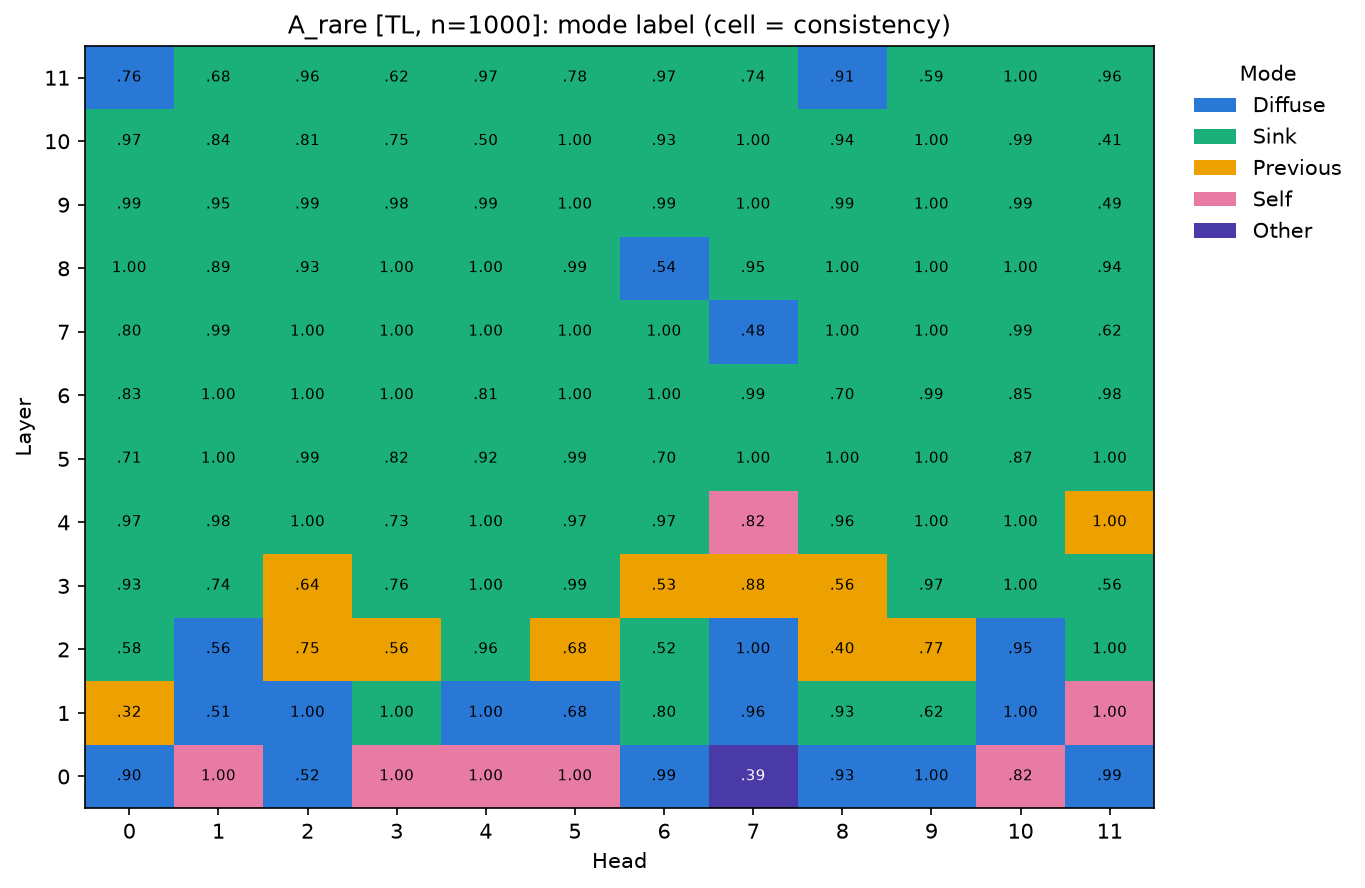
\includegraphics[width=0.53\linewidth]{20260927-235708_exp1/figures/A_rare_mode_label.png}\hfill
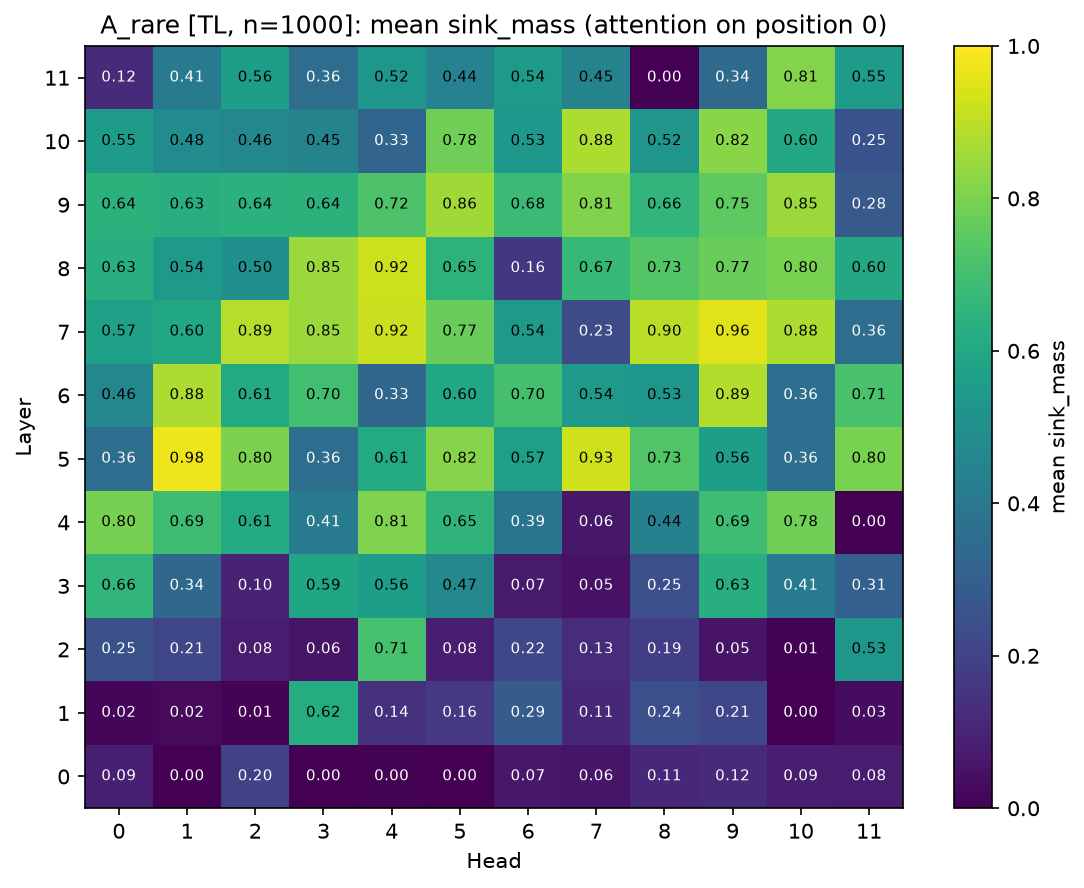
\includegraphics[width=0.43\linewidth]{20260927-235708_exp1/figures/A_rare_sink_mass.png}
\captionof{figure}{Rare-token baseline (1000 sequences). Left: each head's most common label, with the consistency in each cell (\textbf{here green = Sink}; Experiment 2's maps use red for BOS). Right: mean sink mass. 73.6\% of heads are Sink, and layers 5--11 are almost entirely Sink. Layers 0--1 hold diffuse and self-attending heads, and layers 2--4 hold previous-token heads (L4H11: 0.988 of its attention on the previous token). Mean sink mass is 0.33 in layers 0--5 and 0.61 in layers 6--11, peaking in layer 7 (0.70).}
\end{center}
\takeaway{On random tokens, most heads at the final token are idle on BOS, and idling grows with depth. This is the no-op baseline.}

\clearpage
\fig{1.0}{20260928-004336_exp1/figures/phase2_mode_label_panels.png}{The same label map for rare (A), common with byte tokens (B) and byte-free common (C) tokens. The three look almost identical: the share of Sink heads is 73.6\%, 73.6\% and 75.7\%.}

\fig{0.55}{20260928-004336_exp1/figures/phase2_head_types.png}{Head types by condition, with 95\% bootstrap CIs over sequences. The totals barely move.}

\fig{1.0}{20260928-004336_exp1/figures/phase2_sink_mass_diff.png}{But per head, almost everything shifts: 134 of 144 heads differ significantly between A and B (outlined, BH-FDR $q \le 0.05$). Red = less sink on rare tokens: late heads such as L7H7 ($-0.31$). Blue = more sink on rare tokens: early/mid heads such as L2H4 ($+0.35$), L5H2, L10H9. Heads move in opposite directions, so the totals cancel.}

\fig{1.0}{20260928-004336_exp1/figures/phase2_label_shift.png}{Shift in each head's label mix (TV distance; outlined $\ge 0.2$, noise floor 0.09). L7H7 and L10H11 go from Diffuse on rare tokens to Sink on common tokens; several early/mid heads go from Sink to Previous.}
\takeaway{Rare vs common tokens don't change how many heads idle; they change \emph{which} heads idle. Late heads idle more on common tokens, early/mid heads less.}

%=========================== EXP1EXT ===========================
\clearpage
\section{What moves the heads (single-token follow-up, exp1ext)}
For the heads that shifted in Experiment 1, three designs separate where the shift comes from: a 2$\times$2 of context class $\times$ final-token class, a dose-response (replace $k$ of the 31 context tokens), and single-token sweeps at positions 32, 31 and 16. \run{20260928-135243\_exp1ext}

\fig{0.62}{20260928-135243_exp1ext/figures/stage1_interaction_sink_mass.png}{The 2$\times$2 for each tracked head: x = final-token class, line color = context class. Heads whose sink rises from rare to common (blue tags) slope up; heads whose sink falls (orange tags) slope down. Controls (L5H1, L0H1, L4H11) stay flat.}

\clearpage
\begin{center}
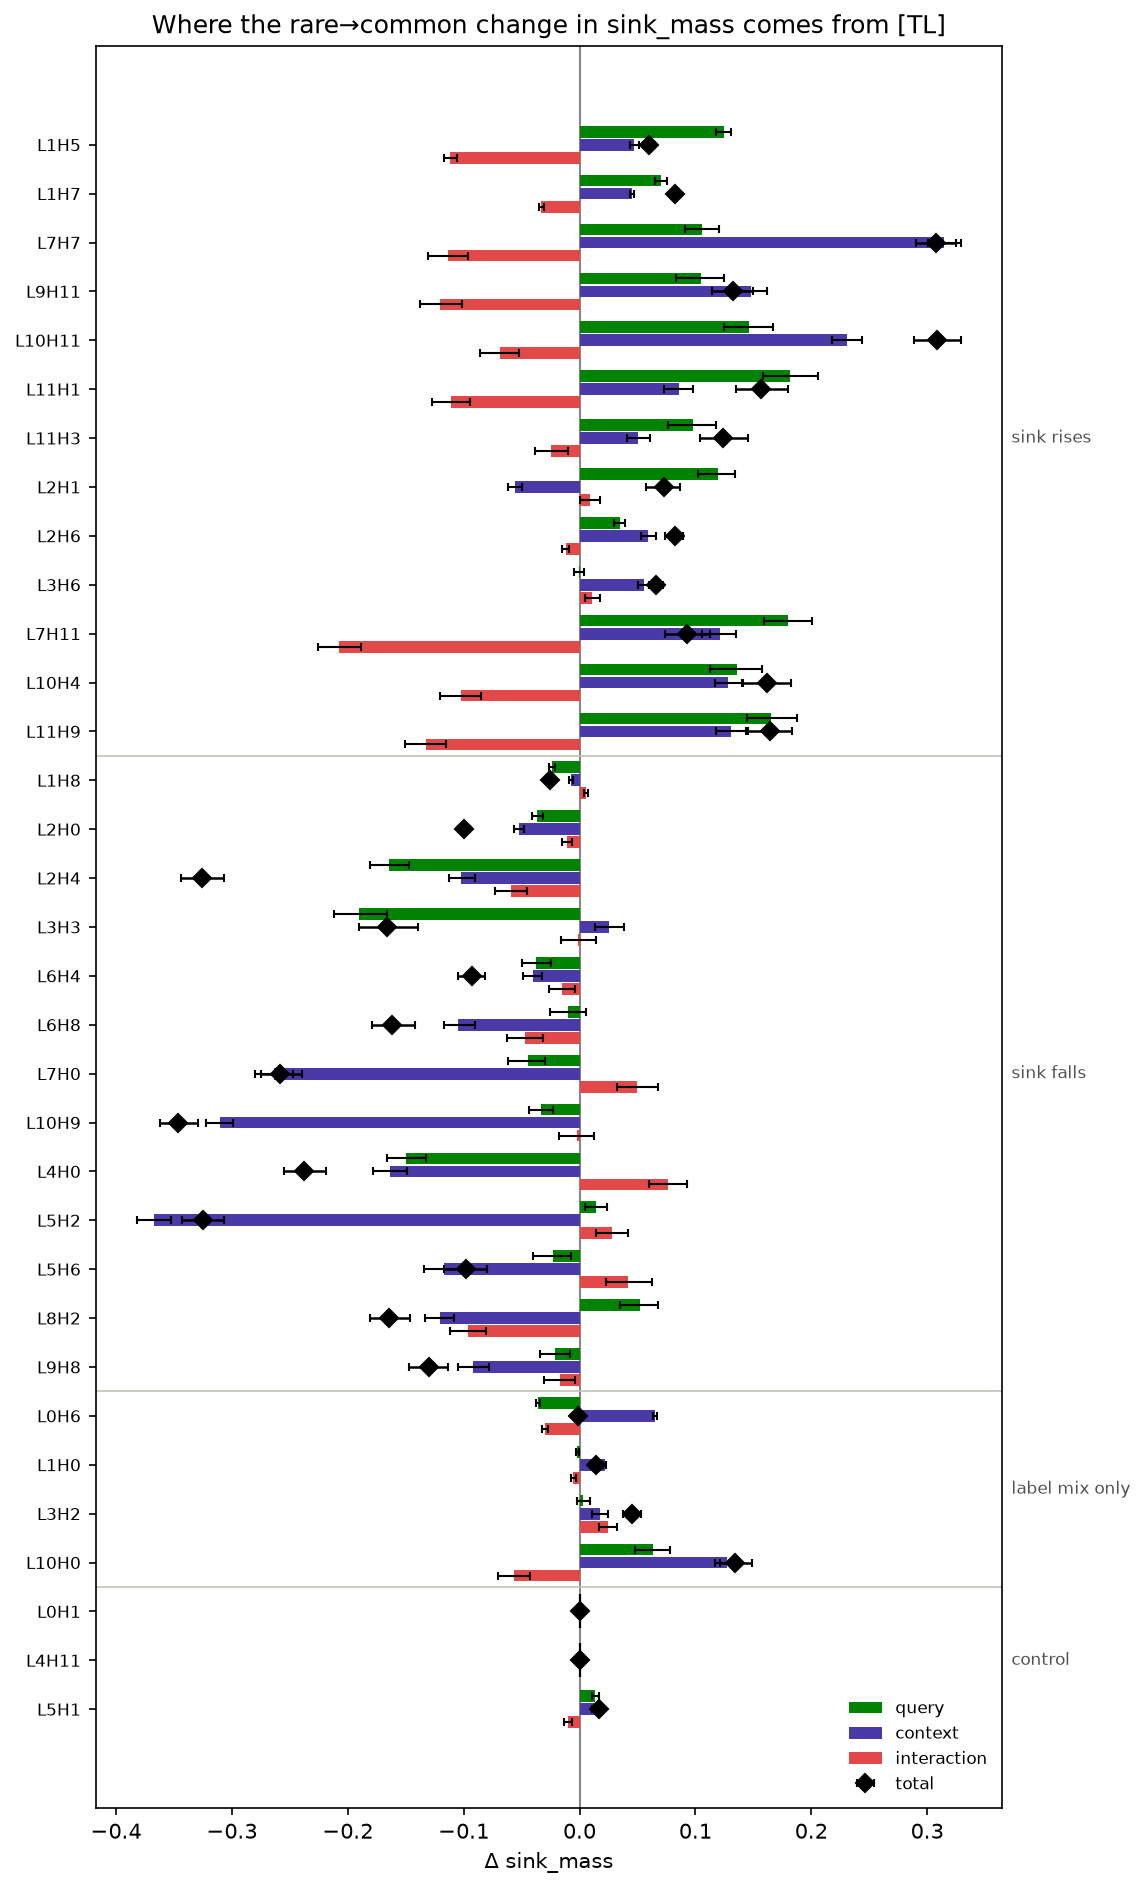
\includegraphics[width=0.42\linewidth]{20260928-135243_exp1ext/figures/stage1_decomposition_sink_mass.png}\hfill
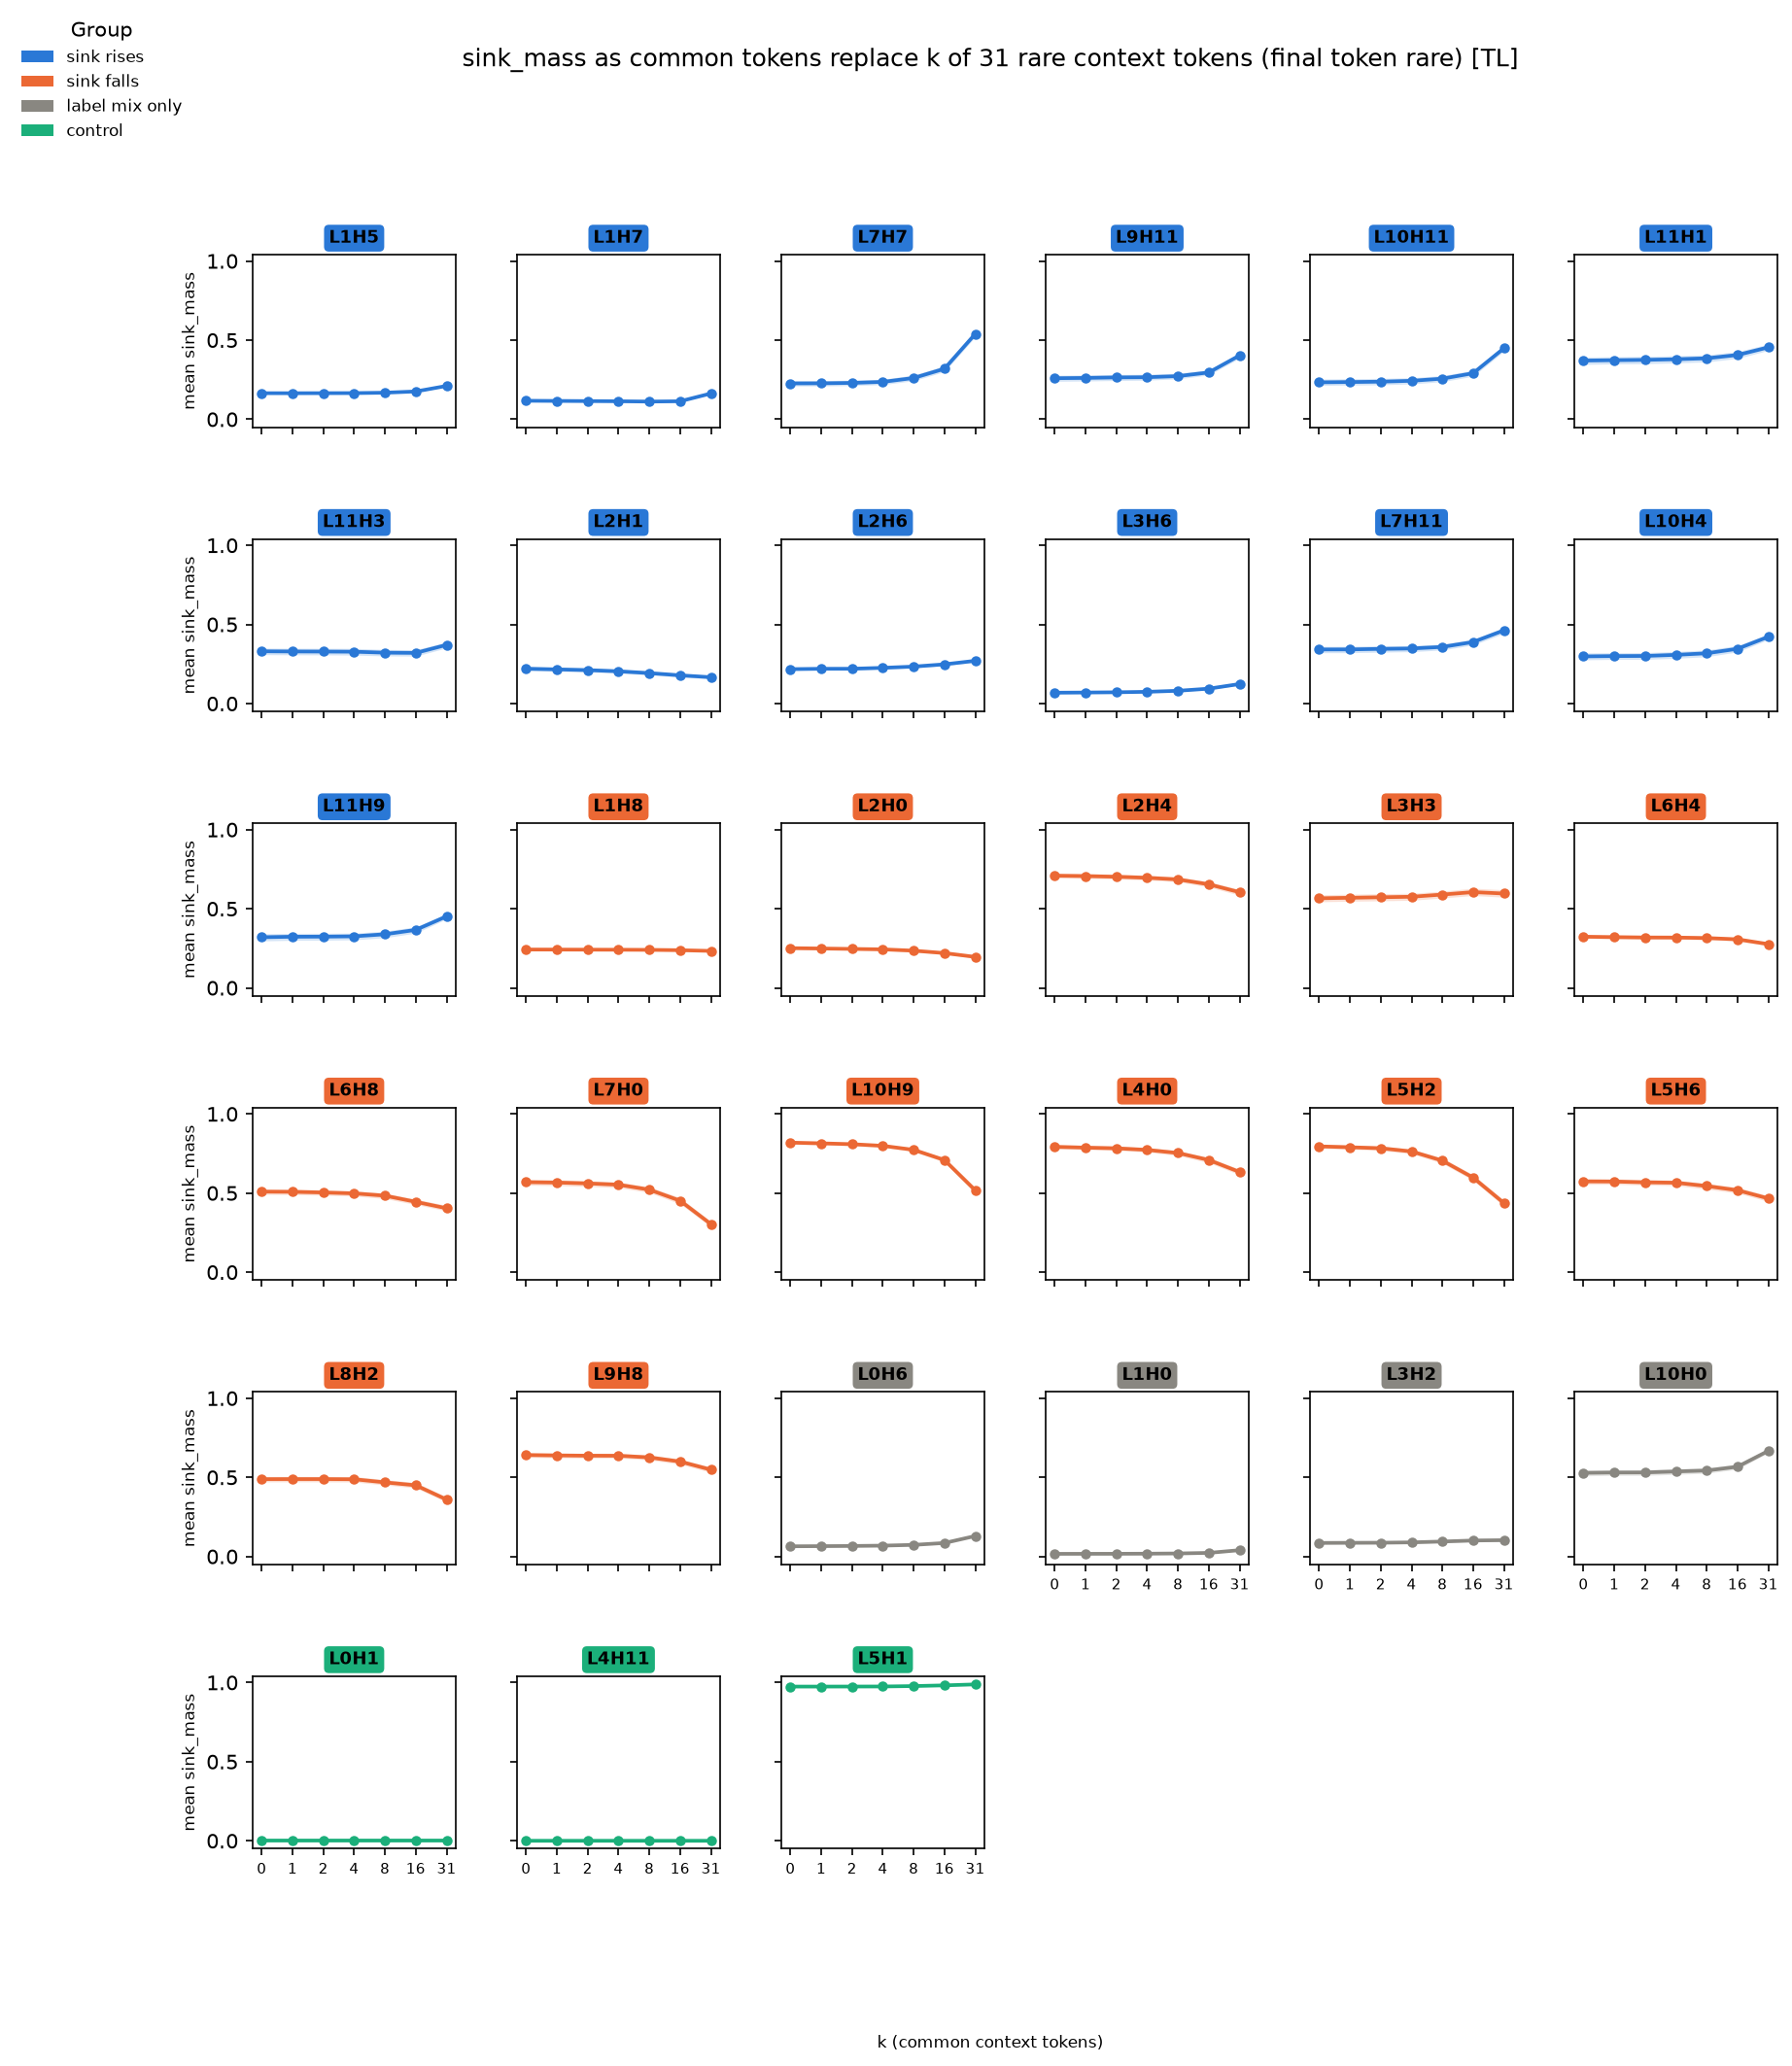
\includegraphics[width=0.55\linewidth]{20260928-135243_exp1ext/figures/stage1_dose_sink_mass.png}
\captionof{figure}{Left: each head's rare$\to$common change split into final token (query), context and interaction. L7H7's change is almost all context ($+0.31$), and L5H2, L10H9 and L7H0 fall through the context ($-0.26$ to $-0.37$). Right: dose-response. Heads stay flat until 16--31 of the 31 context tokens are common (L7H7: 0.22 $\to$ 0.53; L5H2: 0.80 $\to$ 0.43). The whole context matters, not a few tokens.}
\end{center}

\fig{0.78}{20260928-135243_exp1ext/figures/stage2_token_head_heatmap_p31.png}{One token substituted at position 31, right before the final token: strong, token-specific effects. Brackets and punctuation raise L7H7's sink by up to about 0.5, and L2H4, L4H0 and L5H2 fall. The same sweep at position 16 barely moves any head (median per-head spread 0.005 vs 0.029 at position 31).}

\fig{0.82}{20260928-135243_exp1ext/figures/overlay/L7H7.png}{Token-level view of L7H7 on Experiment 1 rows, with each token shaded by the attention the final token pays it. On rare rows it barely parks on BOS (about 0.3); on common rows it does (about 0.5).}
\takeaway{The late-head shift comes from the context as a whole. One token matters only when it sits right before the final token, which set up Experiment 2: write a short phrase exactly there.}

%=========================== EXPERIMENT 2, ITERATION 1 ===========================
\clearpage
\section{Experiment 2: write a phrase into the noise}
Each base row (1000 rare, 1000 common) is overwritten at three positions. Everything else, including the final token, stays the same, so every effect is a within-row difference. \run{20261003-151225\_exp2}

\begin{center}
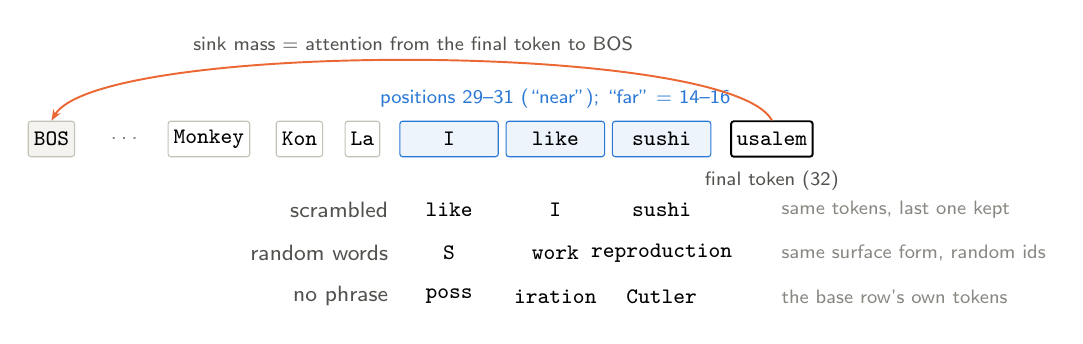
\begin{tikzpicture}[tk/.style={draw=axis,fill=white,rounded corners=1pt,inner sep=2pt,minimum height=0.45cm,font=\ttfamily\footnotesize},
                    sl/.style={tk,draw=cblue,fill=cblue!8,minimum width=1.25cm}]
  \node[tk,fill=plane] (bos) at (0,0) {BOS};
  \node[font=\footnotesize,color=muted] at (0.95,0) {\dots};
  \node[tk] at (2.0,0) {\detokenize{ Monkey}};
  \node[tk] at (3.15,0) {\detokenize{ Kon}};
  \node[tk] at (3.95,0) {La};
  \node[sl] at (5.05,0) {\detokenize{ I}};
  \node[sl] at (6.4,0) {\detokenize{ like}};
  \node[sl] at (7.75,0) {\detokenize{ sushi}};
  \node[tk,draw=black,line width=0.7pt] (q) at (9.15,0) {usalem};
  \node[font=\scriptsize,color=ink2,anchor=north] at (9.15,-0.28) {final token (32)};
  \node[font=\scriptsize,color=cblue,anchor=south] at (6.4,0.27) {positions 29--31 (``near''); ``far'' = 14--16};
  \draw[-{Stealth[length=4pt]},corange,line width=0.7pt] (q.north) .. controls (8.6,1.25) and (0.6,1.25) .. (bos.north)
       node[pos=0.5,above,font=\scriptsize,color=ink2] {sink mass = attention from the final token to BOS};
  \foreach \nm/\x/\y/\z/\note [count=\r] in {scrambled/like/I/sushi/{same tokens, last one kept},
       random words/S/work/reproduction/{same surface form, random ids}, no phrase/poss/iration/Cutler/{the base row's own tokens}} {
    \node[font=\footnotesize,color=ink2,anchor=east] at (4.4,-0.55*\r-0.35) {\nm};
    \node[font=\ttfamily\footnotesize] at (5.05,-0.55*\r-0.35) {\x};
    \node[font=\ttfamily\footnotesize] at (6.4,-0.55*\r-0.35) {\y};
    \node[font=\ttfamily\footnotesize] at (7.75,-0.55*\r-0.35) {\z};
    \node[font=\scriptsize,color=muted,anchor=west] at (9.15,-0.55*\r-0.35) {\note};
  }
\end{tikzpicture}
\captionof{figure}{The design, on a real rare-base row. Contrasts (per row): total = phrase $-$ no phrase; order = phrase $-$ scrambled; identity = scrambled $-$ random words; form = random words $-$ no phrase; placebo = two independent random-word draws (should show nothing). total = order + identity + form exactly.}
\end{center}

\textbf{Color note:} in these contrast maps \textbf{blue = more sink}. The attention maps and token views in Sections 4--5 use the opposite convention, with \textbf{red = more sink}.

\fig{1.0}{20261003-151225_exp2/figures/common_sushi_near_sink_mass_contrasts.png}{Change in sink mass per head for each contrast, common bases, phrase near the final token. Outlined = BH-significant and $|\Delta| \ge 0.02$. Late layers turn blue (more sink) for total, order and identity. Form goes the other way, and the placebo is empty.}

\fig{1.0}{20261003-151225_exp2/figures/rare_sushi_near_sink_mass_contrasts.png}{The same on rare bases: the same direction in late layers, with a smaller order effect.}

\fig{1.0}{20261003-151225_exp2/figures/common_sushi_far_sink_mass_contrasts.png}{The same phrase written mid-sequence (positions 14--16), common bases: much weaker, though not zero (L8H2 $+0.12$).}

\clearpage
\fig{0.85}{20261003-151225_exp2/figures/meaningful_counts_sink_mass.png}{Heads with a meaningful effect per contrast. Near: total 73 (common) / 80 (rare); order 61 / 27. Far: total 37 / 25. Placebo: 0 everywhere.}

\fig{0.78}{20261003-151225_exp2/figures/common_sushi_sink_mass_layer_profile.png}{Where in depth the phrase acts (common bases): mean $|\Delta|$ per layer, by contrast and placement. The near placement dominates from the middle layers up.}
\takeaway{A phrase right before the final token makes late heads idle more. Word order matters (against my prediction), the specific tokens matter more than their surface form, and placing the phrase mid-sequence does little.}

%=========================== ATTENTION MAPS ===========================
\clearpage
\section{Attention maps: Experiment 2 in the style of Experiment 1}
For each variant: mean attention from the final token to BOS (top row), what each head attends to most (middle row; red BOS, blue previous token, yellow another phrase slot, gray other), and the change in BOS attention against no phrase (bottom row; red = more parking). The top two rows look almost the same across variants, because the effect is small (0.01--0.1 per head); the bottom row shows it. The attention was re-extracted from the run's saved rows, and the script checks that it matches the run exactly.

\fig{0.74}{20261003-151225_exp2/figures/attention_maps/common_sushi_near.png}{Common bases, phrase near the final token. With the phrase, layers 5--11 turn broadly red; the scrambled version much less, and random words hardly at all. Heads parking on BOS: 115 with no phrase vs 118 with the phrase.}

\fig{0.74}{20261003-151225_exp2/figures/attention_maps/rare_sushi_near.png}{Rare bases, phrase near the final token. The same pattern, weaker; here the scrambled version comes closer to the phrase.}

\fig{0.74}{20261003-151225_exp2/figures/attention_maps/common_sushi_far.png}{Common bases, phrase mid-sequence (positions 14--16). The change row is much paler.}

\fig{0.74}{20261003-151225_exp2/figures/attention_maps/rare_sushi_far.png}{Rare bases, phrase mid-sequence. The weakest of the four.}
\takeaway{The extra parking is broad: many late heads each shift a little, rather than a few heads flipping category. That's why the label maps barely change while the change maps light up.}

%=========================== TOKEN EFFECTS ===========================
\clearpage
\section{How the tokens move the attention}
\fig{0.6}{20261003-151225_exp2/figures/token_effects/attention_shift_common_near.png}{Where the attention moves, for the 72 late heads (common bases). With the phrase, BOS gains $+0.057$ on average and the rest of the context loses $-0.074$; the token right before the final token (``sushi'') gains $+0.025$. Scrambled: BOS $+0.017$. Random words: $-0.008$. The BOS gain is taken from the random context, not from the phrase.}

\fig{0.6}{20261003-151225_exp2/figures/token_effects/attention_shift_rare_near.png}{The same on rare bases: BOS $+0.025$, taken partly from the phrase tokens themselves (``sushi'' $-0.011$, ``like'' $-0.005$) and partly from the rest ($-0.007$).}

\fig{0.92}{20261003-151225_exp2/figures/token_effects/example_row_rare_L7H0.png}{One real rare-base row, token by token, for head L7H0 (the head with the largest average effect). The row was chosen automatically as the median BOS increase over 1000 rows, not by hand. With the phrase, BOS goes from 0.73 to 0.95 and attention on the token right before the final token falls from 0.17 to 0.02. Scrambled stays at 0.77, random words at 0.70.}

\fig{0.92}{20261003-151225_exp2/figures/token_effects/example_row_common_L7H0.png}{The same head on its median common-base row (BOS increase $+0.23$).}
\takeaway{The coherent phrase pulls late-head attention onto BOS, away from the random context, and for some heads away from the phrase's own last token.}

%=========================== ITERATION 2 ===========================
\clearpage
\section{Iteration 2: more than the sum of its words}
Each phrase word was also written alone at each slot it occupies. Per row, interaction = (phrase $-$ none) $-$ $\Sigma$(each word alone $-$ none), which is zero if the words' effects simply add up. \run{20261003-230841\_exp2}

\fig{1.0}{20261003-230841_exp2/figures/common_sushi_near_additivity.png}{Common bases. For the phrase and the scrambled version: the observed change, the sum of single-word changes, and the interaction (outlined = BH-significant). The phrase's interaction is positive in late layers ($+0.028$ on average); the scrambled version's is negative ($-0.015$).}

\fig{1.0}{20261003-230841_exp2/figures/rare_sushi_near_additivity.png}{Rare bases: phrase interaction $+0.013$, scrambled $+0.004$. Across heads, single-word effects explain essentially none of the order effect ($r^2$ = 0.001 common, 0.007 rare).}

\fig{0.85}{20261003-230841_exp2/figures/surprisal_variants.png}{Does the model's surprise at the phrase explain it? Each point is a variant: mean surprisal of the three slot tokens vs mean late-layer sink. The within-row slope is negative ($-0.0014$ per nat, common) but small: it predicts $+0.005$ of the $+0.040$ order effect. ``sushi'' alone is less predictable yet raises sink, and random words on rare bases are more predictable yet lower it.}
\takeaway{The phrase is more than its words, and the scrambled order is not. Predictability, as the model's own surprisal, explains only about a tenth of it.}

%=========================== ITERATION 3 + TEST C ===========================
\clearpage
\section{Iteration 3 and Test C: it generalizes}
Twelve phrases per template, scrambled by swapping the first two words (last word kept). Bars are each phrase's late-layer interaction with a 95\% CI over rows; filled = CI excludes 0. \run{20261004-125831\_exp2}, \run{20261004-155651\_exp2}, \run{20261004-161908\_exp2}

\fig{0.78}{20261004-125831_exp2/figures/phrase_terms_sink_mass.png}{Pronoun--verb--object (iteration 3). The phrase-minus-scrambled interaction (blue) is positive for 12 of 12 phrases on both bases. Pooled: $+0.025$ common, $+0.010$ rare.}

\fig{0.78}{20261004-125831_exp2/figures/phrase_terms_sink_logit.png}{The same on the logit scale, where effects are not squeezed by the 0--1 bounds: still positive for every phrase ($+0.14$ / $+0.06$ pooled), so this is not a ceiling artifact.}

\clearpage
\fig{0.78}{20261004-155651_exp2/figures/phrase_terms_sink_mass.png}{Adjective--noun--verb (Test C). Common bases: 12 of 12 phrases positive. Rare bases: the order effect is weak (pooled $+0.004$, 6 of 12 phrases, not significant on the logit scale); the scrambled versions also add sink here.}

\fig{0.78}{20261004-161908_exp2/figures/phrase_terms_sink_mass.png}{Preposition--determiner--noun (Test C). 11 of 12 phrases positive on both bases (pooled $+0.013$ common, $+0.017$ rare). All its predictions held.}
\takeaway{In all six template $\times$ base cells, the grammatical phrase adds sink beyond its words and beyond its scrambled version. One cell is inconsistent per phrase (adjective phrases, rare bases), and which base class shows more depends on the template, which is not yet explained.}

%=========================== TEST A ===========================
\clearpage
\section{Test A: the work is done by adjacent word pairs}
For the 12 pronoun--verb--object phrases, each pair of words was also written with the third slot left random. The phrase's interaction splits exactly into three pair terms plus a three-word term. \run{20261004-152303\_exp2}

\fig{1.0}{20261004-152303_exp2/figures/buildup_sink_mass.png}{Each word alone (green), each pair (orange) and the full phrase (blue), as the change in late-layer BOS attention against no phrase. Each bar has a black tick at the sum of its words alone. Bars above their tick do more than their words. The full phrase sits $+1.8$ (rare) and $+2.7$ (common, $\times10^{-2}$) above its tick. The verb--object pair (``like sushi'') carries 61\% / 46\% of that, pronoun--verb 22\% / 34\%, the non-adjacent pair 9\% / 5\%, and the three-word term 8\% / 15\%.}
\takeaway{The effect is local: coherent adjacent word pairs, strongest for the pair ending right before the final token. More familiar verb--object pairs tend to add more, but with 12 phrases that is not significant.}

%=========================== NEXT: TEST B ===========================
\section{Next: Test B, find the circuit}
\textbf{Working hypothesis.} Late heads park on BOS (go no-op) when the words right before the final token form a coherent adjacent pair. Everything so far is behavioural. Test B asks \emph{how}: is the no-op computed by a specific circuit, or a passive fallback? Design and predictions: \texttt{exp2/testb.md}.

\begin{center}
\begin{minipage}[c]{0.4\linewidth}
\centering
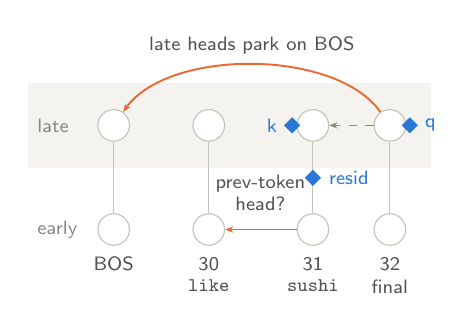
\begin{tikzpicture}[x=1.15cm,y=1.15cm,
    nd/.style={circle,draw=axis,fill=white,inner sep=0pt,minimum size=0.4cm},
    pt/.style={diamond,fill=cblue,inner sep=1.5pt}]
  \fill[plane] (-0.1,0.68) rectangle (4.35,1.62);
  \node[font=\scriptsize,color=muted,anchor=west] at (-0.1,1.15) {late};
  \node[font=\scriptsize,color=muted,anchor=west] at (-0.1,0.0) {early};
  \foreach \nm/\x in {BOS/0.85, 30/1.9, 31/3.05, 32/3.9} {
    \node[nd] (e\nm) at (\x,0) {};
    \node[nd] (l\nm) at (\x,1.15) {};
    \draw[axis,line width=0.4pt] (e\nm) -- (l\nm);
    \node[font=\scriptsize,color=ink2,anchor=north] at (\x,-0.2) {\nm};
  }
  \node[font=\ttfamily\scriptsize,color=ink2,anchor=north] at (1.9,-0.45) {\detokenize{ like}};
  \node[font=\ttfamily\scriptsize,color=ink2,anchor=north] at (3.05,-0.45) {\detokenize{ sushi}};
  \node[font=\scriptsize,color=ink2,anchor=north] at (3.9,-0.45) {final};
  \draw[-{Stealth[length=3pt]},corange,line width=0.7pt] (e31) -- (e30);
  \node[font=\scriptsize,color=ink2,anchor=south,align=center] at (2.47,0.1) {prev-token\\head?};
  \draw[-{Stealth[length=3pt]},corange,line width=0.7pt] (l32) .. controls (3.3,2.0) and (1.45,2.0) .. (lBOS)
       node[pos=0.5,above,font=\scriptsize,color=ink2] {late heads park on BOS};
  \draw[-{Stealth[length=3pt]},muted,dashed,line width=0.5pt] (l32) -- (l31);
  \node[pt] at (3.05,0.57) {}; \node[font=\scriptsize,color=cblue,anchor=west] at (3.12,0.57) {resid};
  \node[pt] at (4.12,1.15) {}; \node[font=\scriptsize,color=cblue,anchor=west] at (4.18,1.15) {q};
  \node[pt] at (2.82,1.15) {}; \node[font=\scriptsize,color=cblue,anchor=east] at (2.76,1.15) {k};
\end{tikzpicture}
\captionof{figure}{Where activations get patched (blue diamonds).}
\end{minipage}\hfill
\begin{minipage}[c]{0.56\linewidth}
\small
Compare ``verb + object'' (\texttt{like sushi}) with ``object alone''; the two runs differ only at position 30. Patch activations from one run into the other:
\begin{enumerate}
  \item residual stream by position $\times$ layer: where the signal lives;
  \item query vs key of the late heads: does the final token ask differently, or do the phrase tokens look different?
  \item single early-head outputs: who writes it;
  \item switch those heads off: does the extra parking disappear?
\end{enumerate}
\textbf{Predictions (written before any data).} B1: the signal moves from position 30 to 31 in early layers. B2: key side over query side. B3: the top writers include a known previous-token head (e.g.\ L4H11, L2H2). B4: switching off the top 3 writers removes $\ge$ 50\% of the effect, while 3 random heads remove $<$ 20\%.
\end{minipage}
\end{center}

\textbf{Why it matters.} It decides whether the no-op state is computed or a fallback, whether idle heads ``find nothing to read'' or ``stop asking'', and it gives Experiment 3 specific heads to switch off or patch in.

\textbf{Limits of everything above.} GPT-2 small only; three hand-picked phrase templates; small effects (late-head mean sink $+0.01$ to $+0.04$); 35 of 43 pre-registered predictions held, and the misses are listed in \texttt{exp2/LOOP\_LOG.md}.

\end{document}
